\let\negmedspace\undefined
\let\negthickspace\undefined
\documentclass[journal]{IEEEtran}
\usepackage[a5paper, margin=10mm, onecolumn]{geometry}
%\usepackage{lmodern} % Ensure lmodern is loaded for pdflatex
\usepackage{tfrupee} % Include tfrupee package

\setlength{\headheight}{1cm} % Set the height of the header box
\setlength{\headsep}{0mm}     % Set the distance between the header box and the top of the text

\usepackage{gvv-book}
\usepackage{gvv}
\usepackage{cite}
\usepackage{amsmath,amssymb,amsfonts,amsthm}
\usepackage{algorithmic}
\usepackage{graphicx}
\usepackage{textcomp}
\usepackage{xcolor}
\usepackage{txfonts}
\usepackage{listings}
\usepackage{enumitem}
\usepackage{mathtools}
\usepackage{gensymb}
\usepackage{comment}
\usepackage[breaklinks=true]{hyperref}
\usepackage{tkz-euclide} 
\usepackage{listings}
% \usepackage{gvv}                                        
\def\inputGnumericTable{}                                 
\usepackage[latin1]{inputenc}                                
\usepackage{color}                                            
\usepackage{array}                                            
\usepackage{longtable}                                       
\usepackage{calc}                                             
\usepackage{multirow}                                         
\usepackage{hhline}                                           
\usepackage{ifthen}
\usepackage{lscape}
\begin{document}

\bibliographystyle{IEEEtran}



\title{4.13.61}
\author{EE25BTECH11057 - Rushil Shanmukha Srinivas
}
% \maketitle
% \newpage
% \bigskip
{\let\newpage\relax\maketitle}

\renewcommand{\thefigure}{\theenumi}
\renewcommand{\thetable}{\theenumi}
\setlength{\intextsep}{10pt} % Space between text and floats

\numberwithin{equation}{enumi}
\numberwithin{figure}{enumi}
\renewcommand{\thetable}{\theenumi}

\textbf{Problem:}A rectangle $PQRS$ has its side $\vec{P}\vec{Q}$ parallel to the line $y = mx$ and vertices $\vec{P}, \vec{Q} \ and \ \vec{S}$ on the lines $y = a, x = b \ and \ x = -b $ ,respectively. Find the locus of the vertex $\vec{R}$.

\textbf{Solution:}
\begin{align}
y=mx \Longrightarrow \vec{n}^\top\vec{x}=0,\vec{n}=\myvec{-m\\1}
\end{align}
The equation of $\vec{P}\vec{Q}$ is $\vec{n}^\top\vec{x}=c$

Let 
\begin{align}
\vec{P}=\myvec{x_1\\a},\vec{Q}=\myvec{b\\y_1},\vec{R}=\myvec{X\\Y},\vec{S}=\myvec{-b\\y_2}
\end{align}
In rectangle diagonals bisect each other
\begin{align}
\vec{P}+\vec{R}=\vec{Q}+\vec{S} \Longrightarrow \myvec{x_1+X\\a+Y}=\myvec{0\\y_1+y_2} 
\end{align}
\begin{align}
x_1=-X, a+Y=y_1+y_2
\end{align}
Also 
\begin{align}
\vec{n}^\top\vec{P}=\vec{n}^\top\vec{Q}=c \Longrightarrow \myvec{-m & 1}\myvec{-X\\a}=\myvec{-m & 1}\myvec{b\\y_1}
\end{align}
\begin{align}
mX+a = -mb+y_1 \Longrightarrow m(X+b)+a=a+Y-y_2
\end{align}
\begin{align}
m(X+b)+y_2 = Y
\end{align}
\begin{align}
\vec{Q}-\vec{P}=\myvec{b+X\\y_1-a},\vec{S}-\vec{P}=\myvec{X-b\\y_2-a}
\end{align}
In  rectangle  PQRS,
\begin{align}
 \vec{P}\vec{Q} \perp \vec{P}\vec{S} \Longrightarrow (\vec{Q}-\vec{P})^\top(\vec{S}-\vec{P})=0 
\end{align}
\begin{align}
\myvec{b+X & Y-y_2}\myvec{X-b\\y_2-a} = 0 
\end{align}
\begin{align}
\myvec{b+X & m(X+b)}\myvec{X-b\\Y-m(X+b)-a} = 0
\end{align}
\begin{align}
(X+b)(X-b+mY-m^2(X+b)-ma) = 0
\end{align}
\begin{align}
X+b = 0 \ or \ (1-m^2)X+mY-(b(1+m^2)+am) = 0
\end{align}
X+b = 0  is not locus of vertex $\vec{R}$ as it gives a fixed point.

The locus is
\begin{align}
(1-m^2)X+mY-(b(1+m^2)+am) = 0
\end{align}

\begin{figure}[h!]
\centering
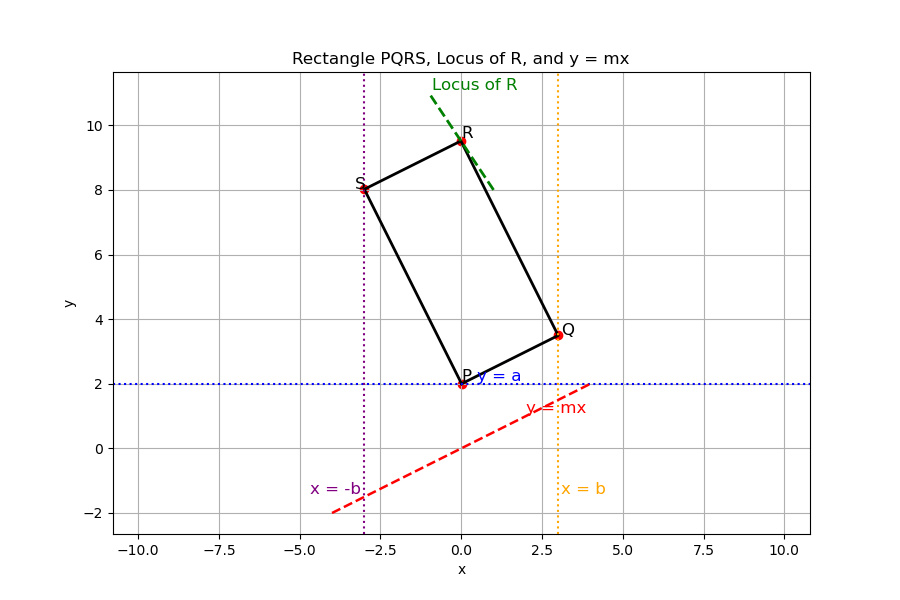
\includegraphics[width=0.9\columnwidth]{figs/locus.png} 
\caption*{Fig: Representation of Rectangle and Locus}
\label{Fig9}
\end{figure}



\end{document}